%%%%%%%%%%%%%%%%%%%%%%%%%%%%%%%%%%%%%%%%%%%%%%%%%%%%%%%%%%%%%%%%%%%%%%%%%%%%%%%

\section{Lecture 1: Introduction to Earth, Richard Gyllencreutz}

Icebreaker Oden:

\begin{figure}[H]
    \centering
    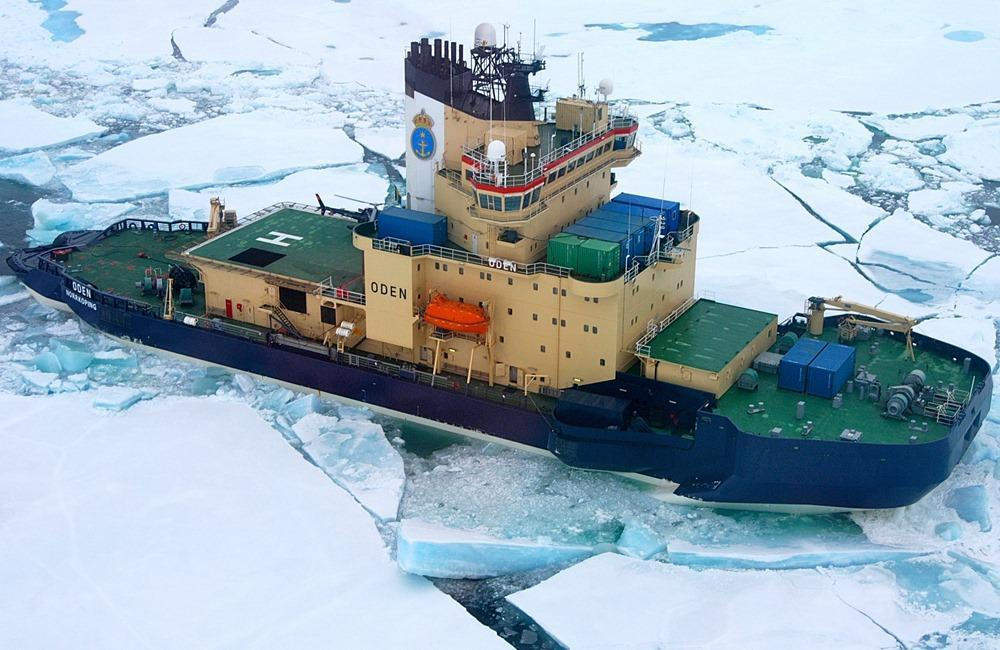
\includegraphics[width=0.9\linewidth]{img/odeb.png}
\end{figure}

\begin{itemize}
    \item The currents around Antarctica are the strongest currents in the
        world.
    \item We've had ice sheets on Antarctica for about 34 Ma.
    \item The hypsographic curve
    \item Hypsometry = area vs. depth/height
    \item Shows the percentage of Earth's surface within a certain range of
        land height or sea depth.
    \item You can use the hypsographic curve to calculate the area of Earth's
        surface over a particular height or elevation range.
    \item For example, about 23\% of the surface is 4km to 5km below sea
        level.
\end{itemize}

\begin{figure}[H]
    \centering
    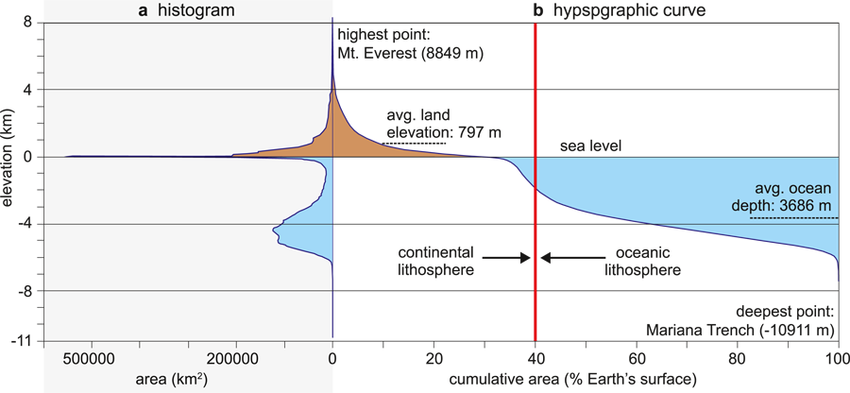
\includegraphics[width=0.9\linewidth]{img/hypsographic_curve.png}
\end{figure}

\begin{itemize}
    \item Solar system -- one star, 4 small rocky planets, 4 gas giants.
    \item The Asteroid belt consists of rock material hindered to become
        planets because of Jupiter's strong gravity. The objects are about
        1 mil km apart, and their total mass is about 3\% of the Moon's.
    \item The Asteroid belt is between the 4 rocky planets and the gas giants.
\end{itemize}

The Earth's internal structure:
\begin{itemize}
    \item Crust, solid, 0 to 7-70km
    \item Mantle, solid but malleable, to 2900km
    \item Outer core, liquid, to 5100km
    \item Inner core, solid, to 6317km
\end{itemize}

The magnetic field:
\begin{itemize}
    \item The core is mostly iron and nickel.
    \item The magnetic field is formed by convection currents in the liquid
        outer core. Earth's rotation $\rightarrow$ aligns the currents and
        magnetic field roughly with the axis.
    \item Sometimes, the magnetic north and south pole switches rapidly
        $\rightarrow$ magnetic pole reversals preserved in rock/sediments
        $\rightarrow$ magnetic time scale.
    \item Highly irregular -- up to millions of years between.
\end{itemize}

\subsection{How do we know the Earth's interior?}
\begin{itemize}
    \item Seismic measurements
    \item Nebular hypothesis
    \item Laboratory experiments
    \item Studies of meteorites
\end{itemize}

\subsubsection{Earthquakes tell us the Earth's inner structure}

Earthquakes can travel as P-waves, S-waves and surface waves.
Only P-waves can travel through fluids. Sound waves are P-waves.

How do we know the inside of Earth? \textbf{Seismic waves}. Knowledge about
Earth's interior is based on many sources of information, but the most
important observations come from \textbf{seismographs} (which produce
\textbf{seismograms}).

Seismographs in different locations show when and where on Earth s-waves and
p-waves are registered from earthquakes (or nuclear bombs).

P-waves are refracted at boundaries between materials with different wave
velocity (refraction by Snell's Law, like for all waves).

\subsubsection{Nebular hypothesis -- collapsing cloud of gas and dust}

\begin{itemize}
    \item Stars are formed in nebulas (clouds of gas and dust) that contracts
        if it contains >80 jupiter masses $\rightarrow$ gravity overcomes
        the gas pressure. The central region $\rightarrow$ the start. The rest
        o the gas and dust $\rightarrow$ the planets.
\end{itemize}

\subsubsection{How do we know about the Earth's interior? Laboratory
experiments}

Lab experiments with diamond anvil cell (DAC) exposes tiny samples to pressures
up to 770 GPa, can be heated by laser to > 5k Celsius, and show how various
materials behave under the extreme conditions inside planets. Because diamond
is transparent to various types of radiation, the sample can be observed
throughout the experiment.

\subsubsection{How do we know about the Earth's interior? Meteorite studies}

The most common are stony meteorites (chondrites and achondrites), iron-stone
meteorites, and iron meteorites. Chondrites contain tiny mineral particles
(chondrules), are about 4.5 Ba old and are thought to represent the original
composition that the stony planets were formed of.

\subsection{Composition of the Earth}

\subsubsection{Crust}

\begin{itemize}
    \item Oxygen: 46\%
    \item Silicon: 28\%
    \item Oxygen: 46\%
    \item Oxygen: 46\%
\end{itemize}

\subsubsection{Mantle}

\begin{itemize}
    \item Oxygen: 44\%
    \item Silicon: 21\%
    \item Magnesium: 22.8\%
    \item Iron: 6.3\%
    \item Calcium: 2.5\%
\end{itemize}

\subsubsection{Outer core}

\begin{itemize}
    \item Iron: 85\%
    \item Oxygen: 5\%
    \item Sulfur: 5\%
    \item Nickel: 5\%
\end{itemize}

\subsubsection{Inner core}

\begin{itemize}
    \item Iron: 94\%
    \item Nickel: 5\%
\end{itemize}

\subsection{How were the oceans formed?}

\begin{itemize}
    \item The primary atmosphere consisted of gases from the planetary
        accretion -- H$_2$, CH$_4$, NH$_3$ (common on the gas giants)
    \item Soon, volcanoes emitted H$_2$O, CO$_2$, N$_2$, and some CO, H$_2$.
    \item Impacts from comets probably also contributed with H$_2$O and
        CO$_2$.
    \item The Earth had cooled enough for liquid water to collect after about
        500 Ma.
    \item The ocean basins are formed by plate tectonics and density
        differences.
    \item Ocean crust is thinner, denser, and "floats" on a deeper level than
        continental crust on the mantle.
    \item Ocean crust is formed at mid-ocean ridges and destroyed in
        subduction zones, and can never become thick. The oldest ocean crust
        is only about 200 Ma.
\end{itemize}

\subsection{Different plate margins, different results}

\begin{itemize}
    \item Convergent plate margin Ocean -- Ocean
    \item Divergent plate margin
    \item Ocean -- Continent
    \item Convergent plate margins
    \item Continent -- Continent
\end{itemize}

\subsection{International Hydrographic Organization (IHO)}

\begin{itemize}
    \item Established in 1921 as the International Hydrographic Bureau (IHB)
    \item In August 2024 the IHO comprised 100 Member States.
    \item Decided the limits of oceans and seas. Hasn't changed since 1953.
\end{itemize}

\subsection{What is a "sea"?}

\begin{itemize}
    \item Composed of salt water, with some exceptions
    \item Smaller and shallower than an ocean
    \item To some extent enclosed by land
    \item Connected to the ocean
\end{itemize}

\subsection{The bathymetry of the world ocean floor}

\begin{itemize}
    \item Lead lines (depth)
    \item Singe beam echo sounder (depth) -- one depth per ping
    \item Multibeam echo sounder (depth, seafloor morphology and
        characteristics). Often called "Swath bathymetry".
    \item Marie Tharp
\end{itemize}

\subsection{The basic principle of echo sounding}

\begin{itemize}
    \item A sound pulse is sent through the water column from a transmitter
        (Tx)
    \item The pulse echoes (is reflected) from the seafloor and is received at
        a receiver (Rx). In simple systems, the Tx and Rx are one and the same
        unit.
    \item The two-way travel time (twt) is registered from when the pulse was
        transmitted until it is received.
\end{itemize}

\subsection{The first bathymetric maps}

\begin{itemize}
    \item Marie Tharp was the first to identify a central valley along the
        mid-ocean ridge -- a major indication that plates are diverging there.
        Fundamental theory for the plate tectonic theory!
\end{itemize}

\subsection{We have only mapped 25\% of the world ocean}

75\% of the oceans floor is only mapped using satellite measurements of sea
surface and gravity.

Sea mount attract water $\rightarrow$ sloping sea surface $\rightarrow$
deflection of gravity.

A challenge with existing mapping technologies is the trade-off between
coverage and resolution.

%%%%%%%%%%%%%%%%%%%%%%%%%%%%%%%%%%%%%%%%%%%%%%%%%%%%%%%%%%%%%%%%%%%%%%%%%%%%%%%